%%=============================================================================
%% LaTeX sjabloon voor bachelorproef, HoGent Bedrijf en Organisatie
%% Opleiding Toegepaste Informatica
%%=============================================================================

\documentclass[fleqn,a4paper,12pt]{book}

%%=============================================================================
%% LaTeX sjabloon voor de bachelorproef, HoGent Bedrijf en Organisatie
%% Opleiding toegepaste informatica
%%
%% Structuur en algemene vormgeving. Meestal hoef je hier niets te wijzigen.
%%
%% Vormgeving gebaseerd op "The Legrand Orange Book", version 2.0 (9/2/15)
%% door Mathias Legrand (legrand.mathias@gmail.com) met aanpassingen door
%% Vel (vel@latextemplates.com). Het oorspronkelijke template is te vinden op
%% http://www.LaTeXTemplates.com
%%
%% Aanpassingen voor HoGent toegepaste informatica: 
%%   Bert Van Vreckem <bert.vanvreckem@hogent.be>
%% Licentie: 
%%   CC BY-NC-SA 3.0 (http://creativecommons.org/licenses/by-nc-sa/3.0/)
%%=============================================================================

%%-----------------------------------------------------------------------------
%% Packages
%%-----------------------------------------------------------------------------

\usepackage[top=3cm,bottom=3cm,left=3cm,right=3cm,headsep=10pt,a4paper]{geometry} % Page margins
\usepackage[utf8]{inputenc}  % Accenten gebruiken in tekst (vb. é ipv \'e)
\usepackage{amsfonts}        % AMS math packages: extra wiskundige
\usepackage{amsmath}         %   symbolen (o.a. getallen-
\usepackage{amssymb}         %   verzamelingen N, R, Z, Q, etc.)
\usepackage[english,dutch]{babel}    % Taalinstellingen: woordsplitsingen,
                             %  commando's voor speciale karakters
                             %  ("dutch" voor NL)
\usepackage{iflang}
\usepackage{eurosym}         % Euro-symbool €
\usepackage{geometry}
\usepackage{graphicx}        % Invoegen van tekeningen
\graphicspath{{img/}}       % Specifies the directory where pictures are stored
\usepackage{tikz}            % Required for drawing custom shapes
\usepackage[pdftex,bookmarks=true]{hyperref}
                             % PDF krijgt klikbare links & verwijzingen,
                             %  inhoudstafel
\usepackage{enumitem}        % Customize lists
\setlist{nolistsep}         % Reduce spacing between list items
\usepackage{listings}        % Broncode mooi opmaken
\usepackage{multirow}        % Tekst over verschillende cellen in tabellen
\usepackage{rotating}        % Tabellen en figuren roteren

\usepackage{booktabs}        % Required for nicer horizontal rules in tables

\usepackage{xcolor}          % Required for specifying colors by name
\definecolor{maincolor}{RGB}{0,147,208} % Define the main color used for 
                             % highlighting throughout the book
                             % 0, 147, 208 = officiële kleur HoGent FBO

% Paragraph style: no indent, add space between paragraphs
\setlength{\parindent}{0em}
\setlength{\parskip}{1em}

\usepackage{etoolbox}
\usepackage{titling} % Macros for title, author, etc
\usepackage{lipsum}          % Voor vultekst (lorem ipsum)

%----------------------------------------------------------------------------------------
%	FONTS
%----------------------------------------------------------------------------------------

\usepackage{avant} % Use the Avantgarde font for headings
%\usepackage{times} % Use the Times font for headings
\usepackage{mathptmx} % Use the Adobe Times Roman as the default text font together with math symbols from the Sym­bol, Chancery and Com­puter Modern fonts

\usepackage{microtype} % Slightly tweak font spacing for aesthetics
\usepackage[utf8]{inputenc} % Required for including letters with accents
\usepackage[T1]{fontenc} % Use 8-bit encoding that has 256 glyphs

%------------------------------------------------------------------------------
%	TITLE PAGE
%------------------------------------------------------------------------------

\newcommand{\inserttitlepage}{%
\begin{titlepage}
  \newgeometry{top=2cm,bottom=1.5cm,left=1.5cm,right=1.5cm}
  \begin{center}

    \begingroup
    \rmfamily
    \includegraphics[width=2.5cm]{img/HG-beeldmerk-woordmerk}\\[.5cm]
    Faculteit Bedrijf en Organisatie\\[3cm]
    \titel
    \vfill
    \student\\[3.5cm]
    Scriptie voorgedragen tot het bekomen van de graad van\\professionele bachelor in de toegepaste informatica\\[2cm]
    Promotor:\\
    \promotor\\
    \ifdefempty{\copromotor}{\vspace{2.5cm}}{Co-promotor:\\\copromotor\\[2.5cm]}
    Instelling: \instelling\\[.5cm]
    Academiejaar: \academiejaar\\[.5cm]
    \ifcase \examenperiode \or Eerste \or Tweede \else Derde \fi examenperiode
    \endgroup

  \end{center}
  \restoregeometry
\end{titlepage}
  \emptypage
\begin{titlepage}
  \newgeometry{top=5.35cm,bottom=1.5cm,left=1.5cm,right=1.5cm}
  \begin{center}

    \begingroup
    \rmfamily
    \IfLanguageName{dutch}{Faculteit Bedrijf en Organisatie}{Faculty of Business and Information Management}\\[3cm]
    \titel
    \vfill
    \student\\[3.5cm]
    \IfLanguageName{dutch}{Scriptie voorgedragen tot het bekomen van de graad van\\professionele bachelor in de toegepaste informatica}{Thesis submitted in partial fulfilment of the requirements for the degree of\\professional bachelor of applied computer science}\\[2cm]
    Promotor:\\
    \promotor\\
    \ifdefempty{\copromotor}{\vspace{2.5cm}}{Co-promotor:\\\copromotor\\[2.5cm]}
    \IfLanguageName{dutch}{Instelling}{Institution}: \instelling\\[.5cm]
    \IfLanguageName{dutch}{Academiejaar}{Academic year}: \academiejaar\\[.5cm]
    \IfLanguageName{dutch}{%
    \ifcase \examenperiode \or Eerste \or Tweede \else Derde \fi examenperiode}{%
    \ifcase \examenperiode \or First \or Second \else Third \fi examination period}
    \endgroup

  \end{center}
  \restoregeometry
\end{titlepage}
}

%----------------------------------------------------------------------------------------
%	BIBLIOGRAPHY AND INDEX
%----------------------------------------------------------------------------------------

\usepackage[style=apa,backend=biber, bibencoding=utf8]{biblatex}
\usepackage{csquotes}
\DeclareLanguageMapping{dutch}{dutch-apa}
\addbibresource{bachproef-tin.bib} % BibTeX bibliography file
\addbibresource{../voorstel/voorstel.bib}
\defbibheading{bibempty}{}

\usepackage{calc} % For simpler calculation - used for spacing the index letter headings correctly
\usepackage{makeidx} % Required to make an index
\makeindex % Tells LaTeX to create the files required for indexing

%----------------------------------------------------------------------------------------
%	MAIN TABLE OF CONTENTS
%----------------------------------------------------------------------------------------

\usepackage{titletoc} % Required for manipulating the table of contents

\contentsmargin{0cm} % Removes the default margin

% Part text styling
\titlecontents{part}[0cm]
{\addvspace{20pt}\centering\large\bfseries}
{}
{}
{}

% Chapter text styling
\titlecontents{chapter}[1.25cm] % Indentation
{\addvspace{12pt}\large\sffamily\bfseries} % Spacing and font options for chapters
{\color{maincolor!60}\contentslabel[\Large\thecontentslabel]{1.25cm}\color{maincolor}} % Chapter number
{\color{maincolor}}
{\color{maincolor!60}\normalsize\;\titlerule*[.5pc]{.}\;\thecontentspage} % Page number

% Section text styling
\titlecontents{section}[1.25cm] % Indentation
{\addvspace{3pt}\sffamily\bfseries} % Spacing and font options for sections
{\contentslabel[\thecontentslabel]{1.25cm}} % Section number
{}
{\hfill\color{black}\thecontentspage} % Page number
[]

% Subsection text styling
\titlecontents{subsection}[1.25cm] % Indentation
{\addvspace{1pt}\sffamily\small} % Spacing and font options for subsections
{\contentslabel[\thecontentslabel]{1.25cm}} % Subsection number
{}
{\ \titlerule*[.5pc]{.}\;\thecontentspage} % Page number
[]

% List of figures
\titlecontents{figure}[0em]
{\addvspace{-5pt}\sffamily}
{\thecontentslabel\hspace*{1em}}
{}
{\ \titlerule*[.5pc]{.}\;\thecontentspage}
[]

% List of tables
\titlecontents{table}[0em]
{\addvspace{-5pt}\sffamily}
{\thecontentslabel\hspace*{1em}}
{}
{\ \titlerule*[.5pc]{.}\;\thecontentspage}
[]

%----------------------------------------------------------------------------------------
%	MINI TABLE OF CONTENTS IN PART HEADS
%----------------------------------------------------------------------------------------

% Chapter text styling
\titlecontents{lchapter}[0em] % Indenting
{\addvspace{15pt}\large\sffamily\bfseries} % Spacing and font options for chapters
{\color{maincolor}\contentslabel[\Large\thecontentslabel]{1.25cm}\color{maincolor}} % Chapter number
{}
{\color{maincolor}\normalsize\sffamily\bfseries\;\titlerule*[.5pc]{.}\;\thecontentspage} % Page number

% Section text styling
\titlecontents{lsection}[0em] % Indenting
{\sffamily\small} % Spacing and font options for sections
{\contentslabel[\thecontentslabel]{1.25cm}} % Section number
{}
{}

% Subsection text styling
\titlecontents{lsubsection}[.5em] % Indentation
{\normalfont\footnotesize\sffamily} % Font settings
{}
{}
{}

%----------------------------------------------------------------------------------------
%	PAGE HEADERS
%----------------------------------------------------------------------------------------

\usepackage{fancyhdr} % Required for header and footer configuration

\pagestyle{fancy}
\renewcommand{\chaptermark}[1]{\markboth{\sffamily\normalsize\bfseries\chaptername\ \thechapter.\ #1}{}} % Chapter text font settings
\renewcommand{\sectionmark}[1]{\markright{\sffamily\normalsize\thesection\hspace{5pt}#1}{}} % Section text font settings
\fancyhf{} \fancyhead[LE,RO]{\sffamily\normalsize\thepage} % Font setting for the page number in the header
\fancyhead[LO]{\rightmark} % Print the nearest section name on the left side of odd pages
\fancyhead[RE]{\leftmark} % Print the current chapter name on the right side of even pages
\renewcommand{\headrulewidth}{0.5pt} % Width of the rule under the header
\addtolength{\headheight}{2.5pt} % Increase the spacing around the header slightly
\renewcommand{\footrulewidth}{0pt} % Removes the rule in the footer
\fancypagestyle{plain}{\fancyhead{}\renewcommand{\headrulewidth}{0pt}} % Style for when a plain pagestyle is specified

% Removes the header from odd empty pages at the end of chapters
\makeatletter
\renewcommand{\cleardoublepage}{
\clearpage\ifodd\c@page\else
\hbox{}
\vspace*{\fill}
\thispagestyle{empty}
\newpage
\fi}

%----------------------------------------------------------------------------------------
%	THEOREM STYLES
%----------------------------------------------------------------------------------------

\usepackage{amsmath,amsfonts,amssymb,amsthm} % For math equations, theorems, symbols, etc

\newcommand{\intoo}[2]{\mathopen{]}#1\,;#2\mathclose{[}}
\newcommand{\ud}{\mathop{\mathrm{{}d}}\mathopen{}}
\newcommand{\intff}[2]{\mathopen{[}#1\,;#2\mathclose{]}}
\newtheorem{notation}{Notation}[chapter]

% Boxed/framed environments
\newtheoremstyle{maincolornumbox}% % Theorem style name
{0pt}% Space above
{0pt}% Space below
{\normalfont}% % Body font
{}% Indent amount
{\small\bf\sffamily\color{maincolor}}% % Theorem head font
{\;}% Punctuation after theorem head
{0.25em}% Space after theorem head
{\small\sffamily\color{maincolor}\thmname{#1}\nobreakspace\thmnumber{\@ifnotempty{#1}{}\@upn{#2}}% Theorem text (e.g. Theorem 2.1)
\thmnote{\nobreakspace\the\thm@notefont\sffamily\bfseries\color{black}---\nobreakspace#3.}} % Optional theorem note
\renewcommand{\qedsymbol}{$\blacksquare$}% Optional qed square

\newtheoremstyle{blacknumex}% Theorem style name
{5pt}% Space above
{5pt}% Space below
{\normalfont}% Body font
{} % Indent amount
{\small\bf\sffamily}% Theorem head font
{\;}% Punctuation after theorem head
{0.25em}% Space after theorem head
{\small\sffamily{\tiny\ensuremath{\blacksquare}}\nobreakspace\thmname{#1}\nobreakspace\thmnumber{\@ifnotempty{#1}{}\@upn{#2}}% Theorem text (e.g. Theorem 2.1)
\thmnote{\nobreakspace\the\thm@notefont\sffamily\bfseries---\nobreakspace#3.}}% Optional theorem note

\newtheoremstyle{blacknumbox} % Theorem style name
{0pt}% Space above
{0pt}% Space below
{\normalfont}% Body font
{}% Indent amount
{\small\bf\sffamily}% Theorem head font
{\;}% Punctuation after theorem head
{0.25em}% Space after theorem head
{\small\sffamily\thmname{#1}\nobreakspace\thmnumber{\@ifnotempty{#1}{}\@upn{#2}}% Theorem text (e.g. Theorem 2.1)
\thmnote{\nobreakspace\the\thm@notefont\sffamily\bfseries---\nobreakspace#3.}}% Optional theorem note

% Non-boxed/non-framed environments
\newtheoremstyle{maincolornum}% % Theorem style name
{5pt}% Space above
{5pt}% Space below
{\normalfont}% % Body font
{}% Indent amount
{\small\bf\sffamily\color{maincolor}}% % Theorem head font
{\;}% Punctuation after theorem head
{0.25em}% Space after theorem head
{\small\sffamily\color{maincolor}\thmname{#1}\nobreakspace\thmnumber{\@ifnotempty{#1}{}\@upn{#2}}% Theorem text (e.g. Theorem 2.1)
\thmnote{\nobreakspace\the\thm@notefont\sffamily\bfseries\color{black}---\nobreakspace#3.}} % Optional theorem note
\renewcommand{\qedsymbol}{$\blacksquare$}% Optional qed square
\makeatother

% Defines the theorem text style for each type of theorem to one of the three styles above
\newcounter{dummy}
\numberwithin{dummy}{section}
\theoremstyle{maincolornumbox}
\newtheorem{theoremeT}[dummy]{Theorem}
\newtheorem{problem}{Problem}[chapter]
\newtheorem{exerciseT}{Exercise}[chapter]
\theoremstyle{blacknumex}
\newtheorem{exampleT}{Example}[chapter]
\theoremstyle{blacknumbox}
\newtheorem{vocabulary}{Vocabulary}[chapter]
\newtheorem{definitionT}{Definition}[section]
\newtheorem{corollaryT}[dummy]{Corollary}
\theoremstyle{maincolornum}
\newtheorem{proposition}[dummy]{Proposition}

%----------------------------------------------------------------------------------------
%	DEFINITION OF COLORED BOXES
%----------------------------------------------------------------------------------------

\RequirePackage[framemethod=default]{mdframed} % Required for creating the theorem, definition, exercise and corollary boxes

% Theorem box
\newmdenv[skipabove=7pt,
skipbelow=7pt,
backgroundcolor=black!5,
linecolor=maincolor,
innerleftmargin=5pt,
innerrightmargin=5pt,
innertopmargin=5pt,
leftmargin=0cm,
rightmargin=0cm,
innerbottommargin=5pt]{tBox}

% Exercise box
\newmdenv[skipabove=7pt,
skipbelow=7pt,
rightline=false,
leftline=true,
topline=false,
bottomline=false,
backgroundcolor=maincolor!10,
linecolor=maincolor,
innerleftmargin=5pt,
innerrightmargin=5pt,
innertopmargin=5pt,
innerbottommargin=5pt,
leftmargin=0cm,
rightmargin=0cm,
linewidth=4pt]{eBox}

% Definition box
\newmdenv[skipabove=7pt,
skipbelow=7pt,
rightline=false,
leftline=true,
topline=false,
bottomline=false,
linecolor=maincolor,
innerleftmargin=5pt,
innerrightmargin=5pt,
innertopmargin=0pt,
leftmargin=0cm,
rightmargin=0cm,
linewidth=4pt,
innerbottommargin=0pt]{dBox}

% Corollary box
\newmdenv[skipabove=7pt,
skipbelow=7pt,
rightline=false,
leftline=true,
topline=false,
bottomline=false,
linecolor=gray,
backgroundcolor=black!5,
innerleftmargin=5pt,
innerrightmargin=5pt,
innertopmargin=5pt,
leftmargin=0cm,
rightmargin=0cm,
linewidth=4pt,
innerbottommargin=5pt]{cBox}

% Creates an environment for each type of theorem and assigns it a theorem text style from the "Theorem Styles" section above and a colored box from above
\newenvironment{theorem}{\begin{tBox}\begin{theoremeT}}{\end{theoremeT}\end{tBox}}
\newenvironment{exercise}{\begin{eBox}\begin{exerciseT}}{\hfill{\color{maincolor}\tiny\ensuremath{\blacksquare}}\end{exerciseT}\end{eBox}}
\newenvironment{definition}{\begin{dBox}\begin{definitionT}}{\end{definitionT}\end{dBox}}
\newenvironment{example}{\begin{exampleT}}{\hfill{\tiny\ensuremath{\blacksquare}}\end{exampleT}}
\newenvironment{corollary}{\begin{cBox}\begin{corollaryT}}{\end{corollaryT}\end{cBox}}

%----------------------------------------------------------------------------------------
%	REMARK ENVIRONMENT
%----------------------------------------------------------------------------------------

\newenvironment{remark}{\par\vspace{10pt}\small % Vertical white space above the remark and smaller font size
\begin{list}{}{
\leftmargin=35pt % Indentation on the left
\rightmargin=25pt}\item\ignorespaces % Indentation on the right
\makebox[-2.5pt]{\begin{tikzpicture}[overlay]
\node[draw=maincolor!60,line width=1pt,circle,fill=maincolor!25,font=\sffamily\bfseries,inner sep=2pt,outer sep=0pt] at (-15pt,0pt){\textcolor{maincolor}{R}};\end{tikzpicture}} % Orange R in a circle
\advance\baselineskip -1pt}{\end{list}\vskip5pt} % Tighter line spacing and white space after remark

%----------------------------------------------------------------------------------------
%	SECTION NUMBERING IN THE MARGIN
%----------------------------------------------------------------------------------------

\makeatletter
\renewcommand{\@seccntformat}[1]{\llap{\textcolor{maincolor}{\csname the#1\endcsname}\hspace{1em}}}
\renewcommand{\section}{\@startsection{section}{1}{\z@}
{-4ex \@plus -1ex \@minus -.4ex}
{1ex \@plus.2ex }
{\normalfont\large\sffamily\bfseries}}
\renewcommand{\subsection}{\@startsection {subsection}{2}{\z@}
{-3ex \@plus -0.1ex \@minus -.4ex}
{0.5ex \@plus.2ex }
{\normalfont\sffamily\bfseries}}
\renewcommand{\subsubsection}{\@startsection {subsubsection}{3}{\z@}
{-2ex \@plus -0.1ex \@minus -.2ex}
{.2ex \@plus.2ex }
{\normalfont\small\sffamily\bfseries}}
\renewcommand\paragraph{\@startsection{paragraph}{4}{\z@}
{-2ex \@plus-.2ex \@minus .2ex}
{.1ex}
{\normalfont\small\sffamily\bfseries}}

%----------------------------------------------------------------------------------------
%	PART HEADINGS
%----------------------------------------------------------------------------------------

% numbered part in the table of contents
\newcommand{\@mypartnumtocformat}[2]{%
\setlength\fboxsep{0pt}%
\noindent\colorbox{maincolor!20}{\strut\parbox[c][.7cm]{\ecart}{\color{maincolor!70}\Large\sffamily\bfseries\centering#1}}\hskip\esp\colorbox{maincolor!40}{\strut\parbox[c][.7cm]{\linewidth-\ecart-\esp}{\Large\sffamily\centering#2}}}%
%%%%%%%%%%%%%%%%%%%%%%%%%%%%%%%%%%
% unnumbered part in the table of contents
\newcommand{\@myparttocformat}[1]{%
\setlength\fboxsep{0pt}%
\noindent\colorbox{maincolor!40}{\strut\parbox[c][.7cm]{\linewidth}{\Large\sffamily\centering#1}}}%
%%%%%%%%%%%%%%%%%%%%%%%%%%%%%%%%%%
\newlength\esp
\setlength\esp{4pt}
\newlength\ecart
\setlength\ecart{1.2cm-\esp}
\newcommand{\thepartimage}{}%
\newcommand{\partimage}[1]{\renewcommand{\thepartimage}{#1}}%
\def\@part[#1]#2{%
\ifnum \c@secnumdepth >-2\relax%
\refstepcounter{part}%
\addcontentsline{toc}{part}{\texorpdfstring{\protect\@mypartnumtocformat{\thepart}{#1}}{\partname~\thepart\ ---\ #1}}
\else%
\addcontentsline{toc}{part}{\texorpdfstring{\protect\@myparttocformat{#1}}{#1}}%
\fi%
\startcontents%
\markboth{}{}%
{\thispagestyle{empty}%
\begin{tikzpicture}[remember picture,overlay]%
\node at (current page.north west){\begin{tikzpicture}[remember picture,overlay]%
\fill[maincolor!20](0cm,0cm) rectangle (\paperwidth,-\paperheight);
\node[anchor=north] at (4cm,-3.25cm){\color{maincolor!40}\fontsize{220}{100}\sffamily\bfseries\@Roman\c@part};
\node[anchor=south east] at (\paperwidth-1cm,-\paperheight+1cm){\parbox[t][][t]{8.5cm}{
\printcontents{l}{0}{\setcounter{tocdepth}{1}}%
}};
\node[anchor=north east] at (\paperwidth-1.5cm,-3.25cm){\parbox[t][][t]{15cm}{\strut\raggedleft\color{white}\fontsize{30}{30}\sffamily\bfseries#2}};
\end{tikzpicture}};
\end{tikzpicture}}%
\@endpart}
\def\@spart#1{%
\startcontents%
\phantomsection
{\thispagestyle{empty}%
\begin{tikzpicture}[remember picture,overlay]%
\node at (current page.north west){\begin{tikzpicture}[remember picture,overlay]%
\fill[maincolor!20](0cm,0cm) rectangle (\paperwidth,-\paperheight);
\node[anchor=north east] at (\paperwidth-1.5cm,-3.25cm){\parbox[t][][t]{15cm}{\strut\raggedleft\color{white}\fontsize{30}{30}\sffamily\bfseries#1}};
\end{tikzpicture}};
\end{tikzpicture}}
\addcontentsline{toc}{part}{\texorpdfstring{%
\setlength\fboxsep{0pt}%
\noindent\protect\colorbox{maincolor!40}{\strut\protect\parbox[c][.7cm]{\linewidth}{\Large\sffamily\protect\centering #1\quad\mbox{}}}}{#1}}%
\@endpart}
\def\@endpart{\vfil\newpage
\if@twoside
\if@openright
\null
\thispagestyle{empty}%
\newpage
\fi
\fi
\if@tempswa
\twocolumn
\fi}

%----------------------------------------------------------------------------------------
%	CHAPTER HEADINGS
%----------------------------------------------------------------------------------------

% A switch to conditionally include a picture, implemented by  Christian Hupfer
\newif\ifusechapterimage
\usechapterimagetrue
\newcommand{\thechapterimage}{}%
\newcommand{\chapterimage}[1]{\ifusechapterimage\renewcommand{\thechapterimage}{#1}\fi}%
\def\@makechapterhead#1{%
{\parindent \z@ \raggedright \normalfont
\ifnum \c@secnumdepth >\m@ne
\if@mainmatter
\begin{tikzpicture}[remember picture,overlay]
\node at (current page.north west)
{\begin{tikzpicture}[remember picture,overlay]
\node[anchor=north west,inner sep=0pt] at (0,0) {\ifusechapterimage\includegraphics[width=\paperwidth]{\thechapterimage}\fi};
\draw[anchor=west] (\Gm@lmargin,-9cm) node [line width=2pt,rounded corners=15pt,draw=maincolor,fill=white,fill opacity=0.5,inner sep=15pt]{\strut\makebox[22cm]{}};
\draw[anchor=west] (\Gm@lmargin+.3cm,-9cm) node {\huge\sffamily\bfseries\color{black}\thechapter. #1\strut};
\end{tikzpicture}};
\end{tikzpicture}
\else
\begin{tikzpicture}[remember picture,overlay]
\node at (current page.north west)
{\begin{tikzpicture}[remember picture,overlay]
\node[anchor=north west,inner sep=0pt] at (0,0) {\ifusechapterimage\includegraphics[width=\paperwidth]{\thechapterimage}\fi};
\draw[anchor=west] (\Gm@lmargin,-9cm) node [line width=2pt,rounded corners=15pt,draw=maincolor,fill=white,fill opacity=0.5,inner sep=15pt]{\strut\makebox[22cm]{}};
\draw[anchor=west] (\Gm@lmargin+.3cm,-9cm) node {\huge\sffamily\bfseries\color{black}#1\strut};
\end{tikzpicture}};
\end{tikzpicture}
\fi\fi\par\vspace*{270\p@}}}

%-------------------------------------------

\def\@makeschapterhead#1{%
\begin{tikzpicture}[remember picture,overlay]
\node at (current page.north west)
{\begin{tikzpicture}[remember picture,overlay]
\node[anchor=north west,inner sep=0pt] at (0,0) {\ifusechapterimage\includegraphics[width=\paperwidth]{\thechapterimage}\fi};
\draw[anchor=west] (\Gm@lmargin,-9cm) node [line width=2pt,rounded corners=15pt,draw=maincolor,fill=white,fill opacity=0.5,inner sep=15pt]{\strut\makebox[22cm]{}};
\draw[anchor=west] (\Gm@lmargin+.3cm,-9cm) node {\huge\sffamily\bfseries\color{black}#1\strut};
\end{tikzpicture}};
\end{tikzpicture}
\par\vspace*{270\p@}}
\makeatother

%----------------------------------------------------------------------------------------
%	HYPERLINKS IN THE DOCUMENTS
%----------------------------------------------------------------------------------------

\usepackage{hyperref}
\hypersetup{hidelinks,backref=true,pagebackref=true,hyperindex=true,colorlinks=false,breaklinks=true,urlcolor= maincolor,bookmarks=true,bookmarksopen=false,pdftitle={Title},pdfauthor={Author}}
\usepackage{bookmark}
\bookmarksetup{
open,
numbered,
addtohook={%
\ifnum\bookmarkget{level}=0 % chapter
\bookmarksetup{bold}%
\fi
\ifnum\bookmarkget{level}=-1 % part
\bookmarksetup{color=maincolor,bold}%
\fi
}
}

%----------------------------------------------------------------------------------------
%	Java source code
%----------------------------------------------------------------------------------------

% Commando voor invoegen Java-broncodebestanden (dank aan Niels Corneille)
% Gebruik:
%   \codefragment{source/MijnKlasse.java}{Uitleg bij de code}
%
% Je kan dit aanpassen aan de taal die je zelf het meeste gebruikt in je
% bachelorproef.
\newcommand{\codefragment}[2]{ \lstset{%
  language=java,
  breaklines=true,
  float=th,
  caption={#2},
  basicstyle=\scriptsize,
  frame=single,
  extendedchars=\true
}
\lstinputlisting{#1}}

% Leeg blad
\newcommand{\emptypage}{%
\newpage
\thispagestyle{empty}
\mbox{}
\newpage
}


%%---------- Documenteigenschappen --------------------------------------------
%% TODO: Vul dit aan met je eigen info:

% Je eigen naam
\newcommand{\student}{Benoit Balliu}

% De naam van je promotor (lector van de opleiding)
\newcommand{\promotor}{Bert Van Vreckem}

% De naam van je co-promotor. Als je promotor ook je opdrachtgever is en je
% dus ook inhoudelijk begeleidt (en enkel dan!), mag je dit leeg laten.
\newcommand{\copromotor}{}

% Indien je bachelorproef in opdracht van/in samenwerking met een bedrijf of
% externe organisatie geschreven is, geef je hier de naam. Zoniet laat je dit
% zoals het is.
\newcommand{\instelling}{HoGent Faculteit Bedrijf en Organisatie}

% De titel van het rapport/bachelorproef
\newcommand{\titel}{Analyse, architectuur en proof-of-concept van een
beveiligde omgeving voor het afnemen van
computerexamens op eigen laptop}

% Datum van indienen (gebruik telkens de deadline, ook al geef je eerder af)
\newcommand{\datum}{31 mei 2019}

% Academiejaar
\newcommand{\academiejaar}{2018-2019}

% Examenperiode
%  - 1e semester = 1e examenperiode => 1
%  - 2e semester = 2e examenperiode => 2
%  - tweede zit  = 3e examenperiode => 3
\newcommand{\examenperiode}{1}

%%=============================================================================
%% Inhoud document
%%=============================================================================

\begin{document}

%---------- Taalselectie ------------------------------------------------------
% Als je je bachelorproef in het Engels schrijft, haal dan onderstaande regel
% uit commentaar. Let op: de tekst op de voorkaft blijft in het Nederlands, en
% dat is ook de bedoeling!

%\selectlanguage{english}

%---------- Titelblad ---------------------------------------------------------
\inserttitlepage

%---------- Samenvatting, voorwoord -------------------------------------------
\usechapterimagefalse
%%=============================================================================
%% Voorwoord
%%=============================================================================

\chapter*{Woord vooraf}
\label{ch:voorwoord}

%% TODO:
%% Het voorwoord is het enige deel van de bachelorproef waar je vanuit je
%% eigen standpunt (``ik-vorm'') mag schrijven. Je kan hier bv. motiveren
%% waarom jij het onderwerp wil bespreken.
%% Vergeet ook niet te bedanken wie je geholpen/gesteund/... heeft

Voor u ligt de bachelorproef: 'Analyse, architectuur en proof-of-concept van een beveiligde omgeving voor het afnemen van computerexamens op eigen laptop.' Het onderzoek hiervoor is in opdracht van Hogeschool Gent gevoerd. Deze bachelorproef is geschreven in het kader van mijn afstuderen aan de opleiding Toegepaste Informatica met afstudeerrichting Systeem- en Netwerkbeheer aan de Hogeschool Gent.

De deelonderzoeksvragen van dit onderzoek zijn opgesteld door mijn promotor en co-promotor Bert Van Vreckem. Bij deze wil ik hem graag bedanken voor de samenwerking en het extra inzicht binnen het examensysteem van Hogeschool Gent dat hij mij aanleverde. 

Verder wil ik een lector die computerexamens afneemt op Hogeschool Gent en een systeembeheerder die bij Hogeschool Gent werkt bedanken voor hun tijd, dankzij hun heb ik de pijnpunten van het huidige systeem en de vereisten van het nieuwe systeem in kaart kunnen brengen.

Tot slot wil ik graag mijn ouders en mijn vriendin bedanken, zij hebben me tijdens dit onderzoek moreel ondersteund en mijn bachelorproef helpen nalezen.

Ik wens u veel leesplezier toe.

Benoit Balliu \\
Gent, 24 mei 2019 
%%=============================================================================
%% Samenvatting
%%=============================================================================

% TODO: De "abstract" of samenvatting is een kernachtige (~ 1 blz. voor een
% thesis) synthese van het document.
%
% Deze aspecten moeten zeker aan bod komen:
% - Context: waarom is dit werk belangrijk?
% - Nood: waarom moest dit onderzocht worden?
% - Taak: wat heb je precies gedaan?
% - Object: wat staat in dit document geschreven?
% - Resultaat: wat was het resultaat?
% - Conclusie: wat is/zijn de belangrijkste conclusie(s)?
% - Perspectief: blijven er nog vragen open die in de toekomst nog kunnen
%    onderzocht worden? Wat is een mogelijk vervolg voor jouw onderzoek?
%
% LET OP! Een samenvatting is GEEN voorwoord!

%%---------- Nederlandse samenvatting -----------------------------------------
%
% TODO: Als je je bachelorproef in het Engels schrijft, moet je eerst een
% Nederlandse samenvatting invoegen. Haal daarvoor onderstaande code uit
% commentaar.
% Wie zijn bachelorproef in het Nederlands schrijft, kan dit negeren, de inhoud
% wordt niet in het document ingevoegd.


%%---------- Samenvatting -----------------------------------------------------
% De samenvatting in de hoofdtaal van het document

\chapter*{Samenvatting}




%---------- Inhoudstafel ------------------------------------------------------
\pagestyle{empty} % No headers
\tableofcontents % Print the table of contents itself
\cleardoublepage % Forces the first chapter to start on an odd page so it's on the right
\pagestyle{fancy} % Print headers again

%---------- Lijst figuren, afkortingen, ... -----------------------------------

% Indien gewenst kan je hier een lijst van figuren/tabellen opgeven. Geef in
% dat geval je figuren/tabellen altijd een korte beschrijving:
%
%  \caption[korte beschrijving]{uitgebreide beschrijving}

\listoffigures
\listoftables

% Als je een lijst van afkortingen of termen wil toevoegen, dan hoort die
% hier thuis. Gebruik bijvoorbeeld de ``glossaries'' package.
% https://www.sharelatex.com/learn/Glossaries

%%---------- Kern -------------------------------------------------------------

%%=============================================================================
%% Inleiding
%%=============================================================================

\chapter{Inleiding}
\label{ch:inleiding}



 Momenteel worden de meeste computerexamens op Hogeschool Gent in een beveiligde omgeving op een computer van de hogeschool afgenomen. Deze methodiek brengt enkele nadelen met zich mee. Het zorgt voor een hoge kost, de hogeschool moet een groot aantal computers te beschikking stellen en deze moeten beschikken over software eigen aan het examen, en monitoringsoftware bevatten zodat examens in een beveiligde omgeving afgelegd kunnen worden. \\ In deze bachelorproef onderzoeken we de haalbaarheid van een beveiligde omgeving waar studenten computerexamens op hun eigen laptop kunnen afleggen. Deze beveilige omgeving moet maximaal vermijden dat fraude mogelijk is. \\


\section{Probleemstelling}
\label{sec:probleemstelling}

Deze bachelorproef is in opdracht van Hogeschool Gent zelf. Het huidige systeem om computerexamens af te nemen op de Hogeschool is verouderd en te duur. Het zorgt voor een grote overhead voor de systeembeheerders en te veel werk voor de docenten zelf. Een systeem dat effici\"{e}nter en meer budgetvriendelijk is moet het huidige systeem vervangen.



\section{Onderzoeksvraag}
\label{sec:onderzoeksvraag}
Is het mogelijk een omgeving, die beveiligd is en voldoet aan de eisen van Hogeschool Gent, op te stellen waar studenten computerexamens op hun eigen laptop kunnen afleggen? 

\subsection{Deelonderzoeksvragen}
\begin{itemize}
	 \item Hoe gebeuren computerexamens nu op de hogeschool? Welke tools worden gebruikt? Welke regels en beperkingen leggen lectoren nu typisch op bij computerexamens?
	
	\item Welke tools/oplossingen bestaan er tegenwoordig voor dit soort situaties? Zijn die voldoende flexibel om bijvoorbeeld een examen programmeren of andere ict-vakken te faciliteren?
	
	\item Als we zelf een omgeving willen opzetten, welke componenten moet die dan bevatten? Welke beperkingen kunnen we studenten opleggen en welk gedrag kunnen we niet vermijden?

\end{itemize} 

\section{Onderzoeksdoelstelling}
\label{sec:onderzoeksdoelstelling}

Het doel van dit onderzoek is om een proof op concept op te stellen die voldoet aan de eisen van de systeembeheerders en de docenten en die een verbetering is tegenover het huidige systeem (op vlak van budget en gebruiksvriendelijkheid). 

\section{Opzet van deze bachelorproef}
\label{sec:opzet-bachelorproef}

% Het is gebruikelijk aan het einde van de inleiding een overzicht te
% geven van de opbouw van de rest van de tekst. Deze sectie bevat al een aanzet
% die je kan aanvullen/aanpassen in functie van je eigen tekst.

De rest van deze bachelorproef is als volgt opgebouwd:

In Hoofdstuk~\ref{ch:stand-van-zaken} wordt een overzicht gegeven van de stand van zaken binnen het onderzoeksdomein, op basis van een literatuurstudie.

In Hoofdstuk~\ref{ch:methodologie} wordt de methodologie toegelicht en worden de gebruikte onderzoekstechnieken besproken om een antwoord te kunnen formuleren op de onderzoeksvragen.

% TODO: Vul hier aan voor je eigen hoofstukken, één of twee zinnen per hoofdstuk
In hoofdstuk~\ref{ch:opstelling} wordt de finale opstelling van het byod-systeem voorgesteld.  

In Hoofdstuk~\ref{ch:conclusie}, tenslotte, wordt de conclusie gegeven en een antwoord geformuleerd op de onderzoeksvragen. Daarbij wordt ook een aanzet gegeven voor toekomstig onderzoek binnen dit domein.


\chapter{Stand van zaken}
\label{ch:stand-van-zaken}

% Tip: Begin elk hoofdstuk met een paragraaf inleiding die beschrijft hoe
% dit hoofdstuk past binnen het geheel van de bachelorproef. Geef in het
% bijzonder aan wat de link is met het vorige en volgende hoofdstuk.

% Pas na deze inleidende paragraaf komt de eerste sectiehoofding.

Voor er onderzoek gedaan wordt naar oplossing voor examens op eigen computer moet er gekeken worden naar de huidige situatie op de Hogeschool Gent en hoe andere instellingen deze probleemstelling aanpakken. 
%Dit hoofdstuk bevat je literatuurstudie. De inhoud gaat verder op de inleiding, maar zal het onderwerp van de bachelorproef *diepgaand* uitspitten. De bedoeling is dat de lezer na lezing van dit hoofdstuk helemaal op de hoogte is van de huidige stand van zaken (state-of-the-art) in het onderzoeksdomein. Iemand die niet vertrouwd is met het onderwerp, weet er nu voldoende om de rest van het verhaal te kunnen volgen, zonder dat die er nog andere informatie moet over opzoeken \autocite{Pollefliet2011}.

\section{Examens op Hogeschool Gent}

\subsection{Soorten examens}
Op Hogent, Faculteit Bedrijf en Organisatie worden er 2 soorten examens afgenomen, mondelinge en schriftelijke. Enkele schriftelijke examens worden enkel op papier afgelegd, anderen deels of volledig op computer. Dit zijn de soorten computerexamens die op HoGent afgenomen worden.
\begin{itemize}
\item Een online test waarbij antwoorden via de webbrowser invgevuld worden (bv. via Chamilo, Cisco-platform, enz.)
\item Een schriftelijk examen waaarbij de voorbereiding op pc gebeurt maar de antwoorden op papier ingevuld worden.
\item Een examen dat op computer m.b.v. specifieke software (bv. IDE en compiler) gemaakt wordt waarna het resultaat digitaal ingediend wordt (bv. Word document met antwoorden, zip-bestand met broncode, Github, ...)
\end{itemize}


\subsubsection{Schriftelijke examens (deels op computer) }

De student heeft toegang tot software (vb. Netbeans, Microsoft Excel, Microsoft Word) en documenten (vb. Examenopgave, Microsoft PowerPoints, PDF-documenten) die zich lokaal bevinden, op vraag van de lector. Deze examens worden altijd op desktops van Hogeschool Gent afgenomen. In een beveiligde gemonitorde omgeving, waarin je enkel kan wat toegestaan is door de docent. De examenopzichter heeft via de admin-computer zicht op alle bureaubladen van de studenten die het examen aan het afleggen zijn. 




\subsubsection{Schriftelijke examens (volledig op computer)}

\paragraph{Examens waarbij toegang tot het gehele systeem vereist is}

Met toegang tot het gehele systeem wordt er bedoeld dat de student hier ook toegang heeft tot software  en documenten die zich lokaal bevinden. Deze examens worden net zoals examens die deels op computer afgenomen worden, altijd op desktops van Hogeschool Gent afgenomen, in diezelfde beveiligde omgeving. Enkel moet de student zijn ingevulde examen digitaal indienen en worden eventuele notities op papier niet bekeken.  

\paragraph{Examens waarbij enkel toegang tot een webbrowser vereist is}

Wanneer er enkel toegang tot een webbrowser vereist is (Test op chamilo, Online-vragenlijst) dan hoeft het examen niet op een desktop van Hogeschool Gent afgelegd te worden. Dit kan ook gewoon via de browser op de laptop van een student. Dit brengt natuurlijk enkele risico's met zich mee, de lector heeft geen zicht op hetgeen de student doet en de student kan communiceren met medestudenten achter de rug van een opzichter. Er kunnen ook bepaalde problemen met de browser opduiken, zoals problemen met plugins en browsertype of browserversie. 

\subsection{Huidige examensysteem}

\subsubsection{Omschrhijving van het huidige systeem}

\subsubsection{Tekortkomingen}

\paragraph{Tekortkomingen volgens docenten}

\paragraph{Tekortkomingen volgens systeembeheerds}

\section{BYOD}

BYOD ofwel Bring Your Own Device is een term die je de laatste jaren wel vaker begint te horen. Door de overvloed van nieuwe apparaten en gadgets, die aan een rotvaart op de markt gebracht worden, is het voor vele bedrijven te duur om altijd mee te zijn met de meest actuele technologiën. De opkomst van BYOD zorgt voor een verschuiving van de overheadkosten, die het beheren van vele apparaten in bezit van het bedrijf met zich meebrengen, weg van het bedrijf naar de werknemers toe \autocite{Hong2016}.

\section{BYOD examens}
Bij BYOD examens leggen studenten examens af op hun eigen laptop. Deze manier van werken is nog niet wijdverspreid. Het kent enkele voor- en nadelen, in de volgende secties zal ik hier wat verder over uitweiden. 

\subsection{Voordelen van BYOD examens}
Het meest prominente voordeel dat BYOD examens met zich meebrengen is het feit dat studenten in een vertrouwde omgeving kunnen werken. Daardoor neemt hun stressgevoeligheid af, volgens
\textcite{TeckSwee2014}. In het onderzoek van \textcite{TeckSwee2014}, waarbij er na een BYOD examen gepolst werd naar de tevredenheid van de deelnemers, was er 74.02\% van de ondervraagde leerlingen (672) meer tevreden met deze manier om examens af te nemen. Dit was in vergelijking met het afleggen van een examen op een computer van de onderwijsinstelling. 

De andere voordelen zijn vooral belangrijk voor de onderwijsinstelling. Doordat de computers uit hun beheer gaan is er een kleinere overhead voor de systeembeheerders en een lagere kost voor de instelling.

\subsection{Opmerkingen bij BYOD examens}

Aangezien examens afleggen op eigen hardware een relatief nieuw gegeven is, ervaren we nog enkele kinderziektes.die problemen kunnen we in 2 groepen indelen. Veiligheid en Werkbaarheid.\\ 

\subsubsection{Problemen op vlak van veiligheid}
Wanneer je niet de volledige controle over een dapparaat hebt kan de mogelijkheid tot fraude niet altijd even makkelijk of zelfs niet vermeden worden.
\textcite{Dawson2016} bekeek in zijn onderzoek 5 manieren om fraude te plegen tijdens een examen op eigen laptop, namelijk: 
\begin{itemize}
	\item De examenopgave lokaal opslaan en achteraf online plaatsen.
	\item Het examen op een virtuele omgeving afleggen en op die manier het besturingssysteem manipuleren
	\item Software aanpassingen maken 

\end{itemize}

Deze methodes zijn gerangschikt in de orde van de kans dat een student tijdens de beperkte examentijd \'{e}\'{e}n van deze methodes toepast. Eerst ga ik wat meer uiteg geven bij de 2 meest gangbare methodes: 

\textbf{De examenopgave lokaal opslaan en achteraf online plaatsen.} De student krijgt de examenopgave lokaal, niets weerhoudt hem dus om daar lokaal een kopie van te maken en om die achteraf (tegen betaling) te verspreiden. Dit zorgt er voor dat de meeste studenten de examens die het jaar ervoor gegeven zijn kunnen inkijken en oplossen of de oplossingen kunnen bekijken. In de snel veranderende wereld van Information Technology hoeft dit geen probleem te zijn, de leerstof kan per jaar vari\"{e}ren. Het betekent natuurlijk wel dat de student de vraagstelling of soort oefeningen die op het examen zal voorkomen beter kan inschatten. Met dit gegeven zal rekeninng gehouden moeten worden bij het opstellen van examens die afgenomen worden op devices van de student. 

\textbf{Het examen op een virtuele omgeving afleggen en op die manier het besturingssysteem manipuleren.} Wanneer er tijdens een computerexamen gemonitord zou worden op systeemvlak, kan een student makkelijk die monitoringsoftware installeren in een virtuele machine en dan op het hostsysteem niet gemonitorde acties uitvoeren (Opzoeken op het internet, communicatie via het internet, opzoeken in lokale documenten). Hierop kan enkel gecontroleerd worden door manueel elke laptop af te gaan om te kijken of de software op de host geinstalleerd is, maar zelfs deze methode is niet waterdicht. Je kan enkel zeker zijn dat de student niet met een virtuele machine werkt wanneer de instelling zelf de software zou installerent. Maar, als devices dan toch beheerd worden door de instelling zelf verlies je de voordelen van het BYOD-principe (minder overhead en minder kosten).

\textbf{software aanpassingen maken.} Aangezien de student de software zelf beheert heeft hij de kans op de software aan te passen, zeker wanneer het open-source software is. Zoals theorie of formules verstoppen in source code. De reden waarom dit zo laag op de lijst staat is omdat het voor een student veel makkelijker is om gewoon een cheat sheet als document te verstoppen op zijn laptop en zo theorie of formules te bekijken. 

\subsubsection{Problemen op vlak van werkbaarheid}
Naast fraude zijn er andere aandachtspunten bij het afnemen van examens op eigen hardware, \textcite{Hillier2015} heeft het in zijn onderzoek over onder andere: laptops die niet sterk genoeg zijn om bepaalde software aan te kunnen, onverwachte crashes van software of besturingssystemen, hardware die tijdens het examen faalt en batterijcapaciteit (indien er geen toegang tot stroom is). Enkele van deze problemen zouden vermeden kunnen worden door minimum hardwarerequirements op te stellen voor laptops en om ervoor te zorgen dat examens altijd in een lokaal met toegang tot netstroom afgenomen worden. Maar zelfs dan kan er niet met 100\% zekerheid gezegd worden dat er geen hardware of software faalt tijdens die examens. Hetzelfde kan natuurlijk gezegd worden voor desktops van de instelling zelf, maar dan ligt de verantwoordelijkheid bij de instelling, niet bij de student. 


    
\section{BYOD Systemen}

Het invoeren van BYOD examens kan op verschillende manieren. Daarom is er in samenspraak met Bert Van Vreckem een scope vastgesteld voor dit onderzoek. De implementatie van BYOD examens moet hetzelfde zijn en mogelijk zijn voor de 3 meest gangbare besuringssystemen (Linux, MacOs en Windows) en het is niet de bedoeling, dat een student specifieke software moet installeren (voor monitoring of internet filtering e.d.). Deze scope limiteert het aantal mogelijke implementaties. In dit onderzoek bekijken we 4 manieren om BYOD examens te faciliteren, namelijk:

\begin{itemize}
\item Safe Exam Browser 
\item Televic AssessmentQ / AVIDAnet Lite
\item Desktop virtualisatie via een cloudprovider
\item Beveiligde, configureerbare netwerkomgeving om internettoegang tot niet-toegestane sites vanop laptops te vermijden	
\end{itemize}


%Je verwijst bij elke bewering die je doet, vakterm die je introduceert, enz. naar je bronnen. In \LaTeX{} kan dat met het commando \texttt{$\backslash${textcite\{\}}} of \texttt{$\backslash${autocite\{\}}}. Als argument van het commando geef je de ``sleutel'' van een ``record'' in een bibliografische databank in het Bib\TeX{}-formaat (een tekstbestand). Als je expliciet naar de auteur verwijst in de zin, gebruik je \texttt{$\backslash${}textcite\{\}}.
%Soms wil je de auteur niet expliciet vernoemen, dan gebruik je \texttt{$\backslash${}autocite\{\}}. In de volgende paragraaf een voorbeeld van elk.

%\textcite{Knuth1998} schreef een van de standaardwerken over sorteer- en zoekalgoritmen. Experten zijn het erover eens dat cloud computing een interessante opportuniteit vormen, zowel voor gebruikers als voor dienstverleners op vlak van informatietechnologie~\autocite{Creeger2009}.




%%=============================================================================
%% Methodologie
%%=============================================================================

\chapter{Methodologie}
\label{ch:methodologie}

%% TODO: Hoe ben je te werk gegaan? Verdeel je onderzoek in grote fasen, en
%% licht in elke fase toe welke stappen je gevolgd hebt. Verantwoord waarom je
%% op deze manier te werk gegaan bent. Je moet kunnen aantonen dat je de best
%% mogelijke manier toegepast hebt om een antwoord te vinden op de
%% onderzoeksvraag.

\section{Fasering}

De rest van dit onderzoek is uitgevoerd in 3 delen, namelijk: 
\begin{itemize}
	\item Eerst is er onderzocht welke oplossingen er reeds bestaan voor dergelijke systemen, en hoe dit best opgesteld wordt in de proof-of-concept.
	\item Dan zijn er een aantal mogelijke opstellingen gemaakt en met elkaar vergeleken.
	\item Uiteindelijk is er een proof-of-concept opgesteld, rekeninghoudend met de bevindingen uit de tweede fase.
\end{itemize}

\section{Onderzoek naar mogelijke oplossingen}
Nu er beslist is welk systeem er opgezet wordt voor de proof-of-concept is het belangrijk op te lijsten hoe het onderzoek verder verloopt. Hieronder vindt u een oplijsting van technologie\"{e}n die gebruikt kunnen worden bij de uiteindelijke opstelling van het bring-your-own-device systeem met beveiligde netwerkomgeving.

\subsection{GNS3}
GNS3 ofwel Graphical Network Simulator 3 is een network software emulator. Deze software staat toe om virtuele en fysieke apparaten met elkaar te verbinden om zo complexe netwerken te simuleren. GNS3 kan virtuele machines van VMWare, VirtualBox of KVM gewoon importeren en routeren. Dankzij GNS3 was het testen van een opstelling tijdens het onderzoek een stuk makkelijker en kon het opstellen van een proof-of-concept versneld worden.

\subsubsection{Tekortkoming}
Wireless access points zijn niet ondersteund binnen GNS3. Voor de proof-of-concept is er dus gebruik gemaakt van een opstelling met wired connections. In de realiteit verkiezen we dus wireless access omdat niet alle moderne laptops nog een ethernetpoort hebben.   

\subsection{Virtualisatie van overige apparaten}
Om de virtualisatie van niet-netwerk apparaten, zoals end devices te faciliteren is er gebruik gemaakt van VMWare. Gebruik van Virtualbox machines of machines op een KVM Server is ook mogelijk. 


\subsection{Open-source software}
Omdat de opstelling open-source moest blijven is er voor de opstelling enkel naar open source netwerk operating systems/software gekeken. Onder andere:
\begin{itemize}	
	\item pfSense: Open-source operating system gebaseerd op FreeBSD. Router/firewall.
	\item OpenWrt: Open-source Linux operating system. Volledige netwerk oplossing. 
	\item dnsmasq: Open-source Unix-like operating system. DNS forwarder en DHCP Server.
\end{itemize}


\subsection{Automatisatie}

Om het opstellen van dergelijke omgeving zo simpel mogelijk te maken is er gekozen om een groot stuk te automatiseren d.m.v. Ansible. Ansible is Agentless SSH automation. Dit wil zeggen dat er op de nodes die je beheert met ansible geen speciale software moet draaien, enkel een OpenSSH server die standaard geinstalleerd is op de meeste systemen. Met Ansible en haar netwerk modules kan je makkelijk volledige netwerkomgevingen opzetten zonder zelf aan de command-line interface te moeten wijzigenn. 

\section{Mogelijke opstellingen maken}
Voor er een goede finale opstelling opgezet kan worden moeten er een aantal opstellingen met elkaar vergeleken worden. Hier volgt een lijst van opstellingen die suboptimaal bleken na onderzoek:
\begin{itemize}
	\item \textbf{Opstelling waarbij de netwerkinfrastructuur uit ciscoapparatuur bestaat}. Na het opzetten van die opstelling in GNS3 bleek deze suboptimaal. Dergelijk systeem is heel erg duur en voor het beperkt aantal gebruikers dat op hetzelfde moment met de apparatuur moet verbinden zou cisco-infrastructuur onnodig zijn. Cisco levert enterprise-grade infrastructuur, in dit geval is die apparatuur ongeschikt. 
	\item \textbf{Opstelling met OpenWRT router}. OpenWRT is gemaakt om op veel kleinere en minder krachtige apparaten te werken. Bij het opzetten van een OpenWRT omgeving was het duidelijk dat de configuratie van de router niet zo gebruiksvriendelijk is. Aangezien het de bedoeling is dat lectoren zelf de omgeving beheren is het gebruik van OpenWRT niet aangeraden. 
	\item \textbf{Opstelling met pfSense Router zonder Ansible}. Het gebruik van pfSense als router software maakt het opstellen van de netwerkomgeving een stuk makkelijker. Lectoren die omgeving volledig zelf laten opzetten is niet haalbaar.  
	 
\end{itemize} 

\section{Proof-of-concept}
Na het configureren van die vorige opstellingen is er \'{e}\'{e}n uitgekozen, namelijk degene die het best voldoet aan de vastgestelde vereisten. Daarover kan u in het volgende hoofdstuk lezen.

\chapter{Proof of concept}
\label{ch:proofofconcept}



\section{Opstelling}

De opstelling van de  proof of concept, die u terug kan vinden op \hyperref[fig:Poc1]{figuur 4.1}, bestaat uit:
\begin{itemize}
	\item pfSense router en firewall
	\item CentOS server met een dnsmasq DNS en DHCP Server
	\item CentOS server met Gitlab Community Edition ge\"{\i}nstalleerd.
	\item Switch
	\item End devices (laptops)
\end{itemize}

Opmerking: bij gebrek aan ondersteuning van open-source Wireless Access Points binnen GNS3, zijn de laptops van de studenten bedraad verbonden met het netwerk. Bij een echte opstelling is het de bedoeling dat er een Captive Portal geconfigureerd wordt op de pfSense Router zodat enkel studenten met toestemming kunnen verbinden. PfSense routers ondersteunen o.a. LDAP Authenticatie, waarmee je gebruikers met hun Microsoft Active Directory Account kan authenticeren om in te loggen op het netwerk.   
	
\begin{figure}
	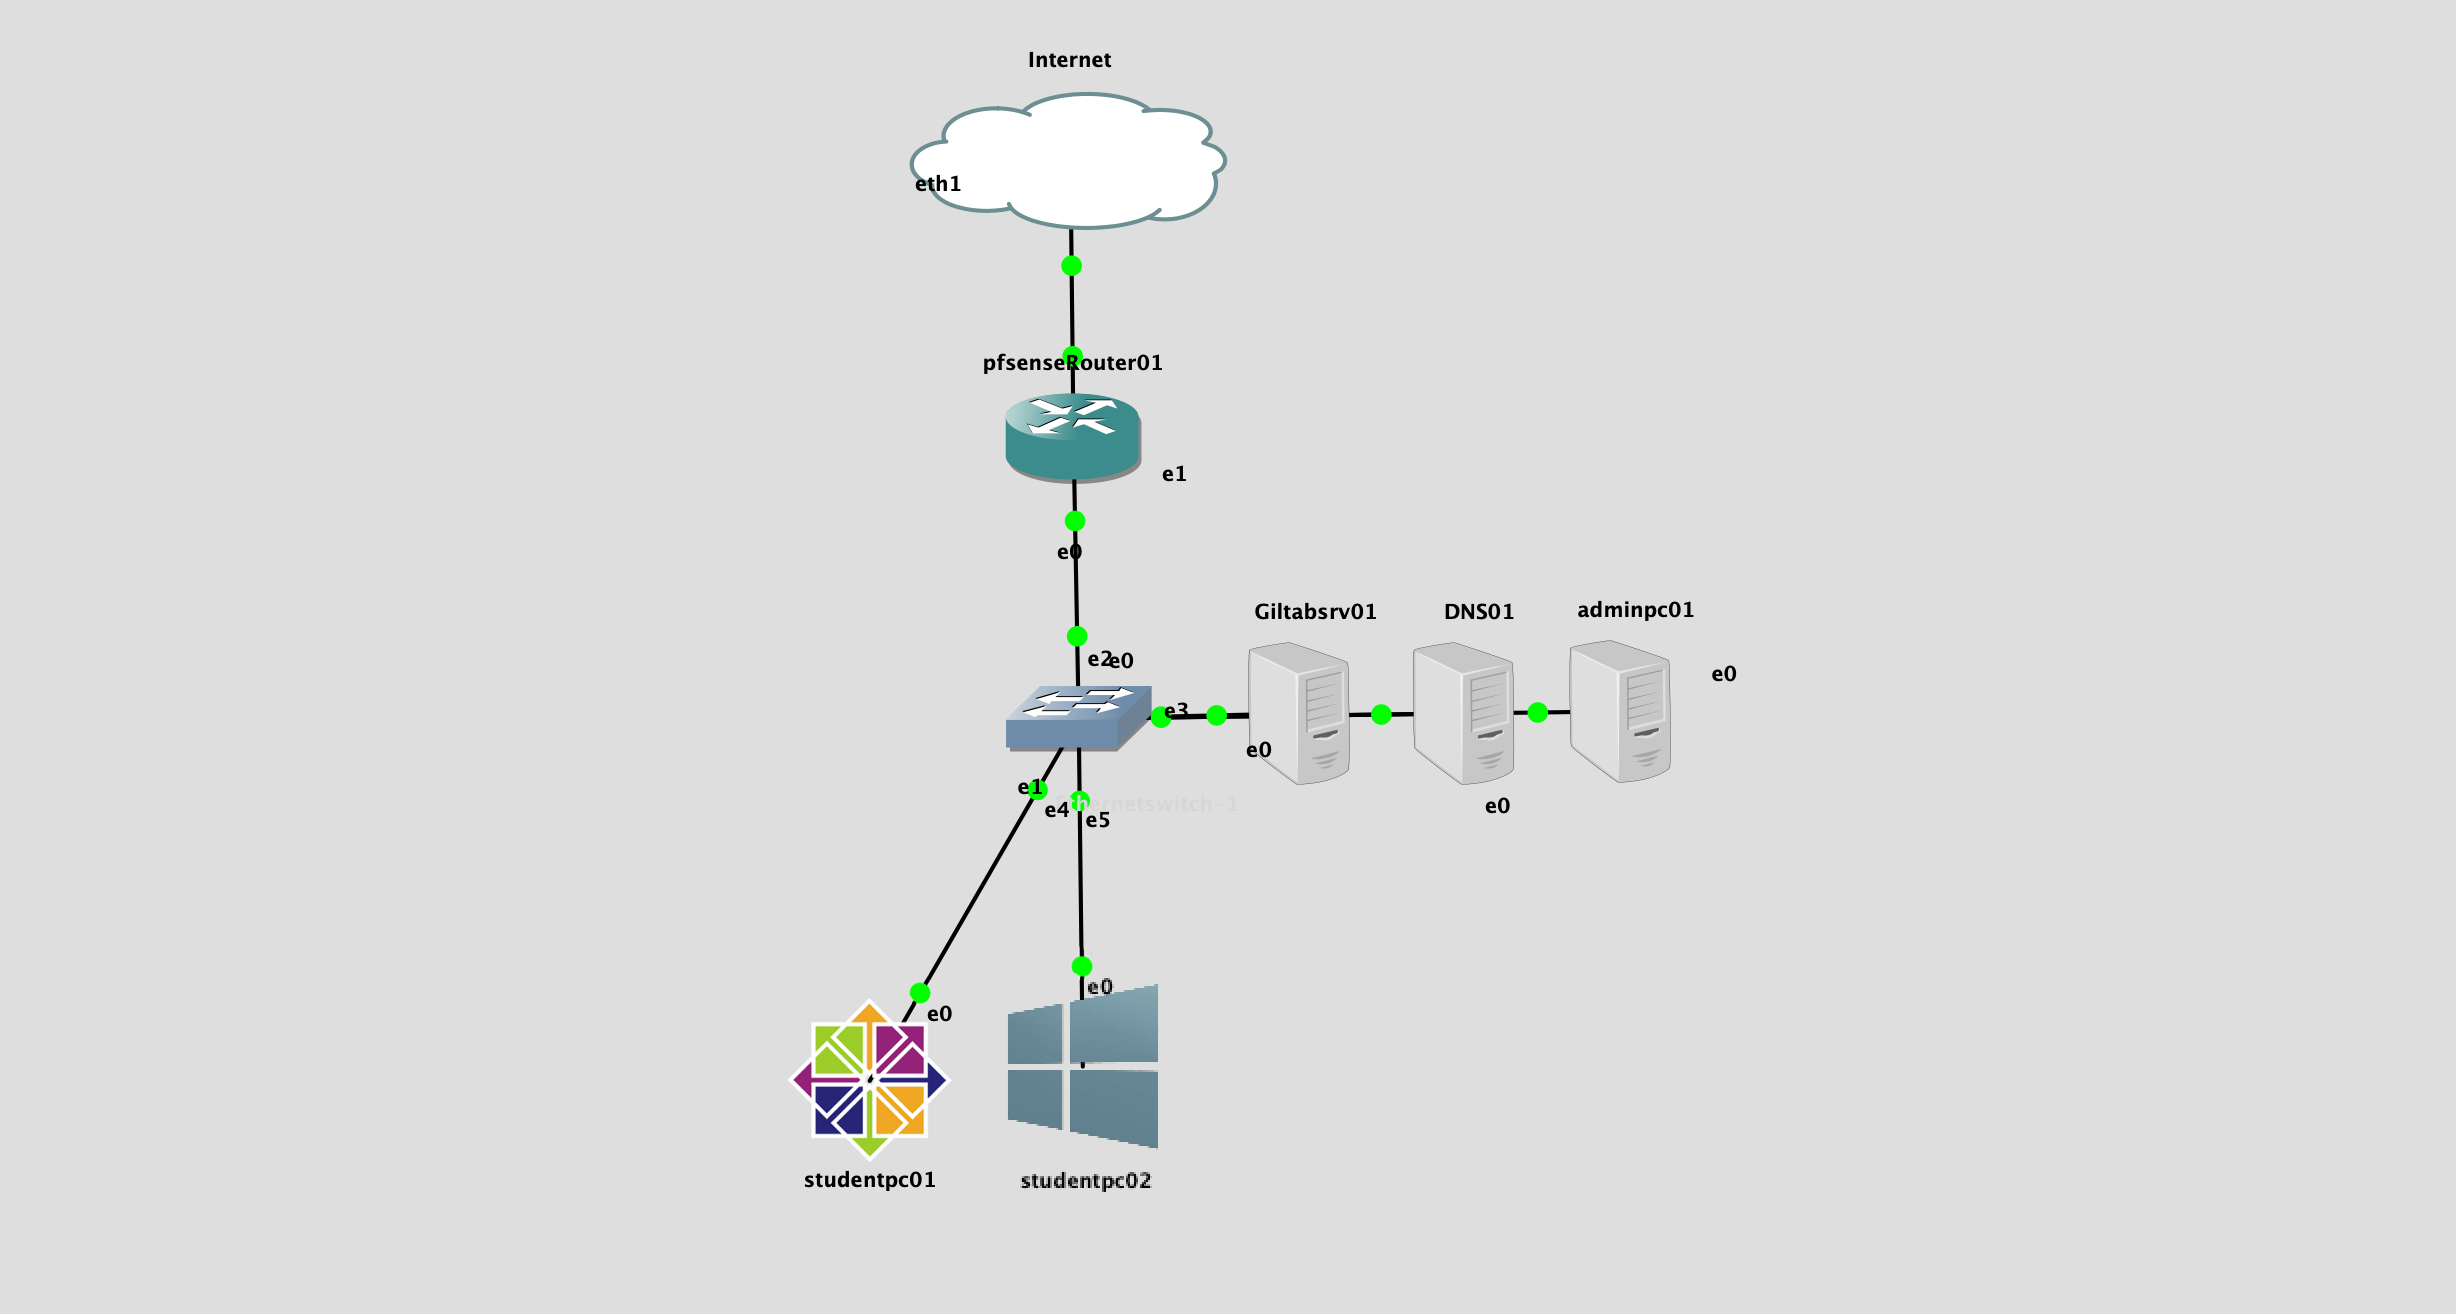
\includegraphics[width=\linewidth]{img/gns3FinalPoC.jpg}
	\caption{Opstelling voorgesteld in GNS3}
	\label{fig:PoC1}
\end{figure}

\subsection{Functionaliteiten}

Hier volgt een opsomming van alle functionaliteiten die een dergelijke opstelling bevat.

\begin{itemize}
	\item Alle admin systemen zijn gehardened en beveiligd volgens een Baseline gebaseerd op de CIS Guidelines.
	\item De het opzetten van de omgeving voor een examen wordt grotendeels door Ansible gedaan.
	\item Het is simpel om de examenomgeving op te zetten voor een lector (dankzij Ansible). 
	\item De studenten kunnen enkel browsen naar websites die toegestaan zijn door de lecoren.
	\item Beveiliging op zowel de firewall en DNS zorgen ervoor dat studenten geen VPN-verbinding kunnen maken of een andere DNS Server kunnen gebruiken.
	\item Studenten kunnen hun examen van de lokale Gitlab server halen en na het examen indienen via Gitlab
	\item Er wordt gemonitord of studenten niet met andere netwerken verbinden.
\end{itemize}

\subsection{Ontbrekende functionaliteiten}

Deze proof of concept is geen ideale oplossing voor het nieuwe examensysteem, het is wel de meest ideale oplossing binnen dit onderzoek.
Toch blijft er een functionaliteit over die voor sommige examens een nice-to-have is en voor andere een must-have, namelijk: 

Studenten hebben volledige toegang tot documenten op hun eigen laptop. Indien zij reeds gemaakte oefeningen, opgeloste voorbeeldexamens of vorige versies van examens bij zouden hebben, is het mogelijk dat zij een oneerlijk voordeel krijgen tegenover studenten die dit niet bijhebben. Volgens een lector die programmeerexamens afneemt, maakt dat voor examens zoals Object-Geori\"{e}nteerd Programmeren III minder uit vergeleken met Object-Geori\"{e}nteerd Programmeren I, waar het die lector noodzakelijk is dat studenten geen toegang hebben tot alle oefeningen, bijvoorbeeld.

\subsection{Automatisatie}
Automatisatie gebeurt met Ansible. Ansible communiceert met de servers via SSH met 4096bit SSH keys. Het is niet mogelijk om op die servers met een wachtwoord in te loggen.

\subsubsection{DNS \& Firewall}
Wanneer studenten toch websites mogen bezoeken zoals bijvoorbeeld de java api, moet er een aanpassing gemaakt worden in DNS en Firewall. Wanneer de lector de URL van een site ingeeft bij het uitvoeren van de ansible playbook, worden de juiste aanpassingen gemaakt op beide servers.

\subsection{Gitlab}
Gebruikers worden in deze proof-of-concept via de Gitlab API toegevoegd met Ansible. Wanneer de docent gebruikers aanlevert in een .csv bestand, dan leest Ansible die uit en voegt ze toe aan de Gitlab server. 

Dit is de Ansible taak die per student in die .csv file uitgevoerd wordt. De waarden die tussen: "\{\{\}\}"   staan, zijn variabelen die per student verschillend zijn.
\lstset{basicstyle=\ttfamily}
\begin{lstlisting}
-  name: Create Gitlab User
	gitlab_user:
		server_url: https://gitlabsrv01.benoitballiu.be
		validate_certs: True
		api_username: admin
		api_password: $encrypted$
		group: "{{ group }}"
		access_level: developer
		name: "{{ studentName }}"
		username: "{{ username }}"
		email: "{{ studentEmail }}"
		password: dummypassword
		state: present
	delegate_to: localhost
\end{lstlisting}

Het volledige Ansible Playbook kan u in de bijlagen terugvinden.

\section{Verloop van een examen}
Deze sectie geeft meer uitleg over BYOD-examen met deze opstelling, door een voorbeeld van het verloop te geven.

\subsection{Voorbeeld: Examen OOPII}

\begin{itemize}
	\item De lector bereidt de avond voor het examen of op de dag zelf het examen voor, door een een Ansible Playbook te doorlopen. Ansible zal zo users, studenten die het examen afleggen, toevoegen aan zowel de gitlabserver als de Captive portal van de router en, indien gewild, url's te whitelisten. Zie figuur \hyperref[fig:PoC2]{4.2}, dit is het scherm dat de lector invult. Zowel figuur \hyperref[fig:PoC3]{4.3} als figuur \hyperref[fig:PoC4]{4.4} voor een voorbeeld van de files die de lector moet invullen. 

	\begin{figure}[H]
		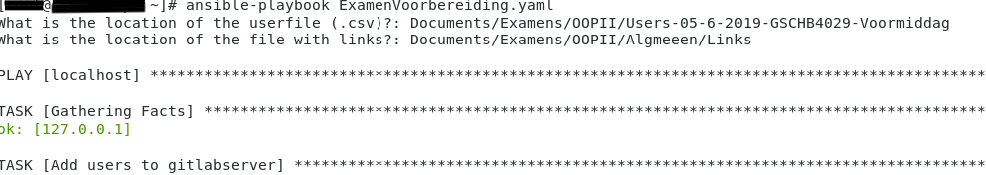
\includegraphics[width=\linewidth]{img/AdminPC.png}
		\caption[Voorbeeld van het Ansible Playbook]{Dit is hoe een docent een examen voorbereidt. een lector geeft hier de locaties van de gevraagde bestanden in.}
		\label{fig:PoC2}
	\end{figure}
	
	\begin{figure}[H]
	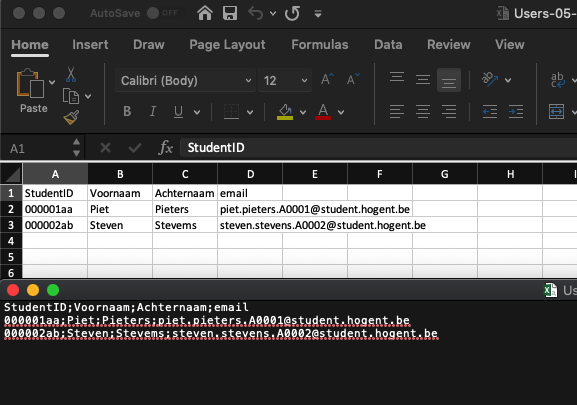
\includegraphics[width=\linewidth]{img/CSV1.png}
	\caption[Voorbeeld van Users.csv]{Boven zie je een voorbeeld van een User file die een lector invult, onder zie je dezelfde file op de manier dat Ansible hem inleest.}
	\label{fig:PoC3}
\end{figure}

	\begin{figure}[H]
	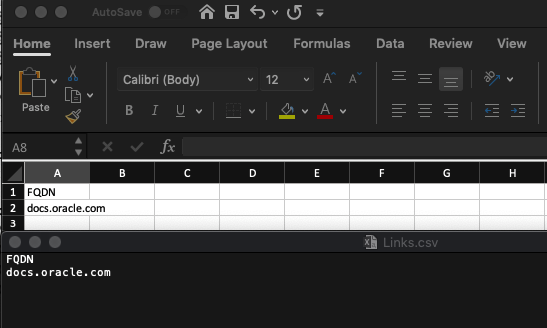
\includegraphics[width=\linewidth]{img/CSV2.png}
	\caption[Voorbeeld van Links.csv] {Boven zie je een voorbeeld van een Link file die een lector invult, onder zie je dezelfde file op de manier dat Ansible hem inleest.}
	\label{fig:PoC4}
\end{figure}

	\item De lector kan op de adminmachine testen of de studenten enkel aan de toegestane url's kunnen.
	
		\begin{figure}[H]
		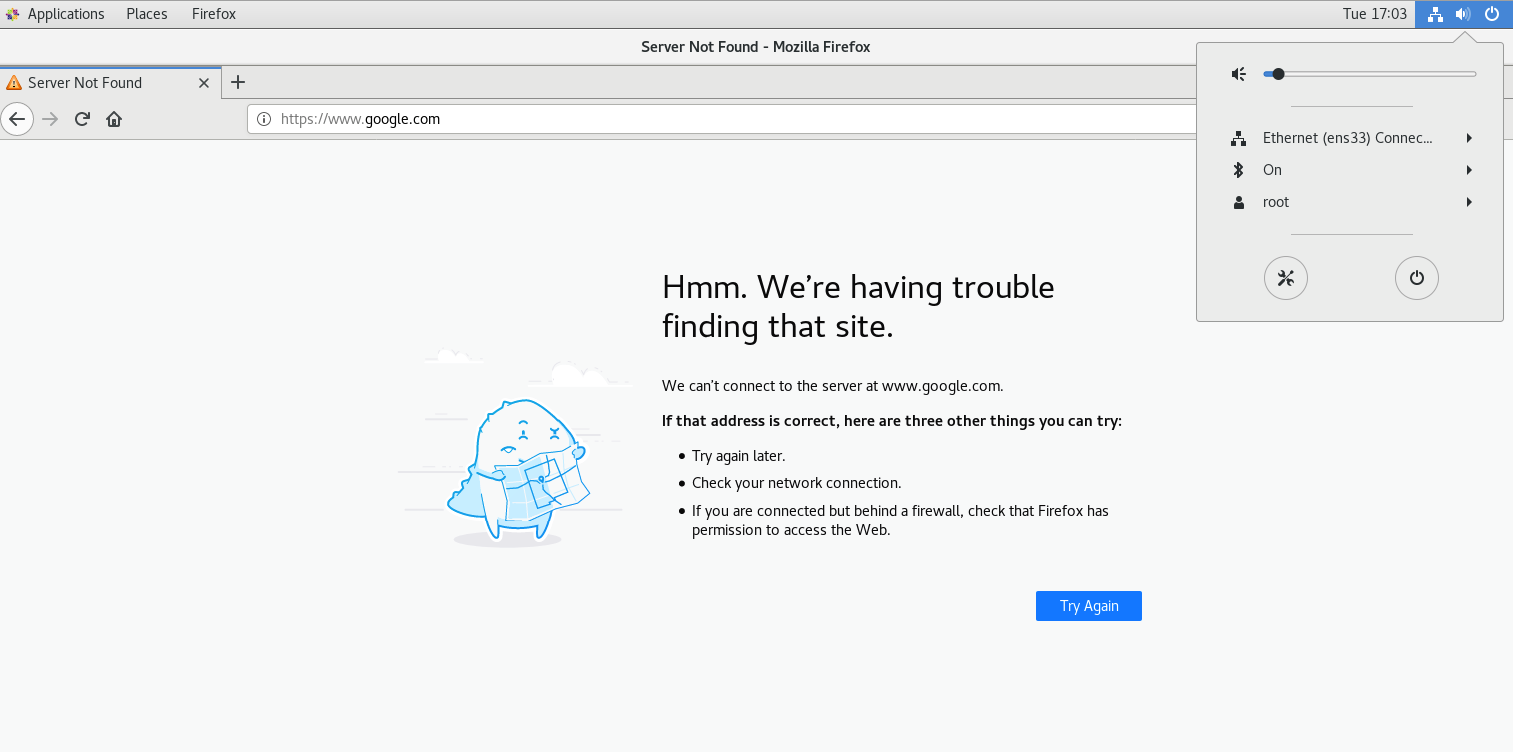
\includegraphics[width=\linewidth]{img/Linkblock1.png}
		\caption[Screenshot van webbrowser 1] {Hierboven zie je een screenshot van wat er gebeurt wanneer de docent een site verschillend van de toegelaten sites uittest.}
		\label{fig:PoC5}
	\end{figure}

		\begin{figure}[H]
		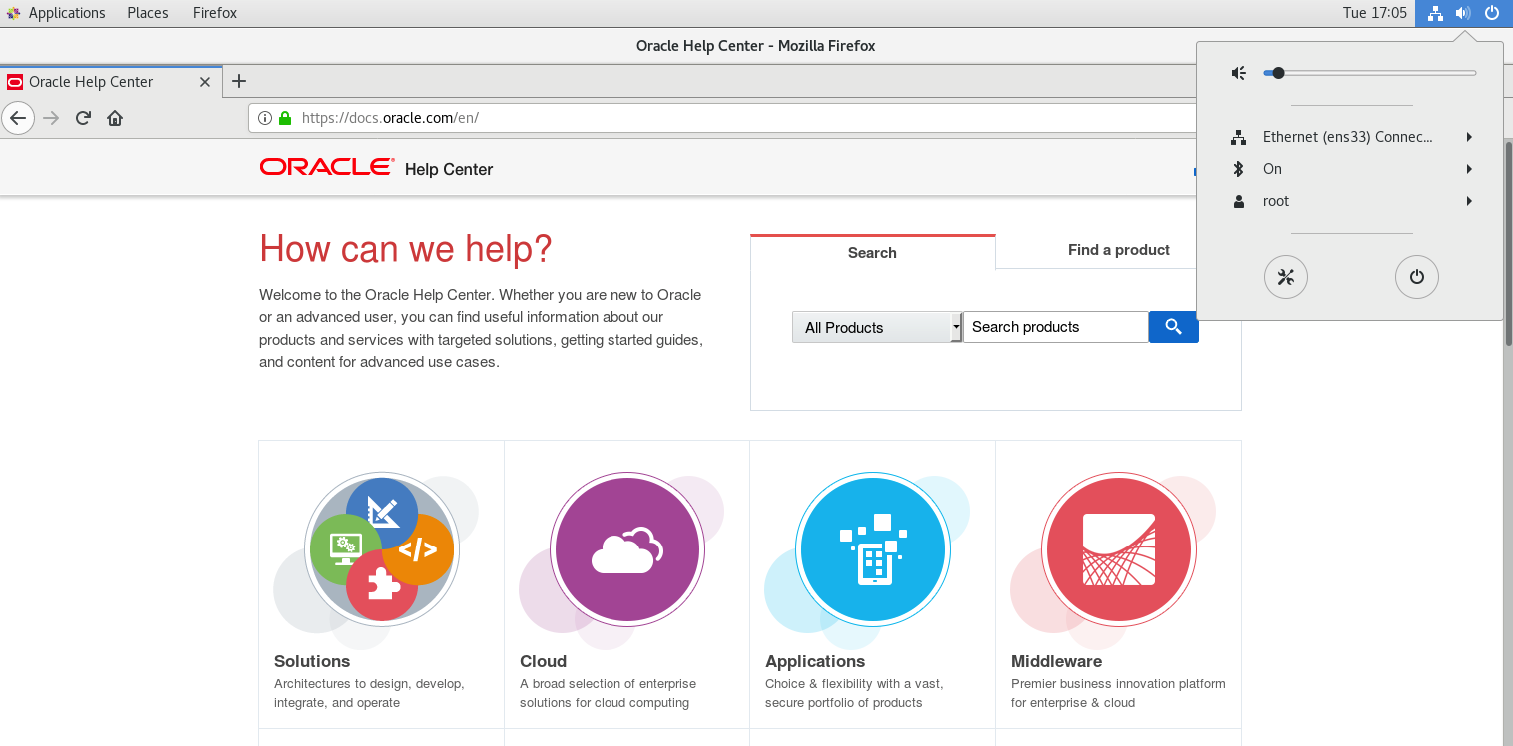
\includegraphics[width=\linewidth]{img/Linkblock2.png}
		\caption[Screenshot van webbrowser 2] {Hierboven zie je een screenshot van wat er gebeurt wanneer de docent één van de toegestane sites uittest.}
		\label{fig:PoC6}
	\end{figure}
	\item De lector voegt zijn project toe aan Gitlab. Dit kan hij manueel doen: 
			\begin{figure}[H]
		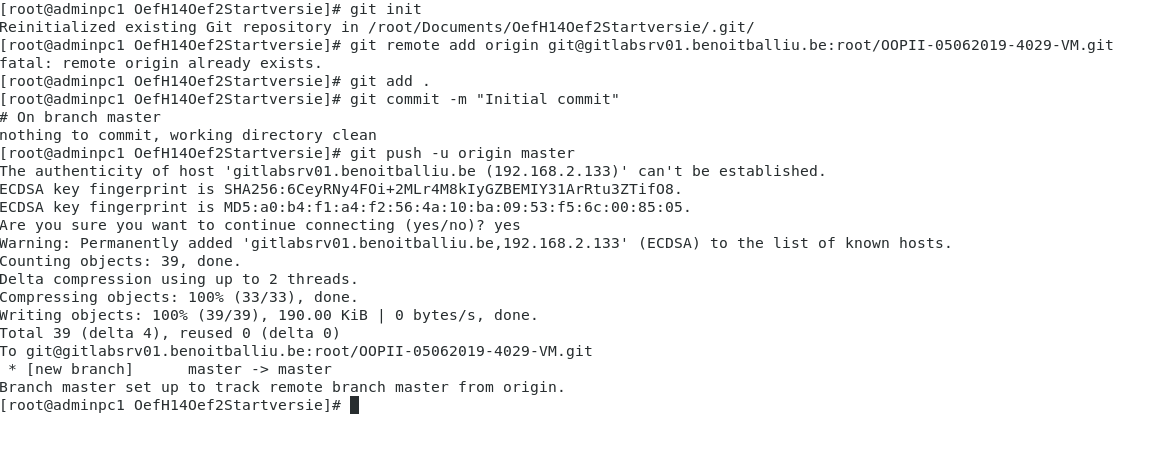
\includegraphics[width=\linewidth]{img/Git01.png}
		\caption[Screenshot van het aanmaken van een git repository] {Hierboven zie je een screenshot waar een lector een nieuw repository toegvoegt aan de gitlabserver.}
		\label{fig:PoC7}
	\end{figure}
    Gezien het thema van automatisatie is dit in het eindelijke playbook toch geautomatiseerd. 
   			\begin{figure}[H]
   	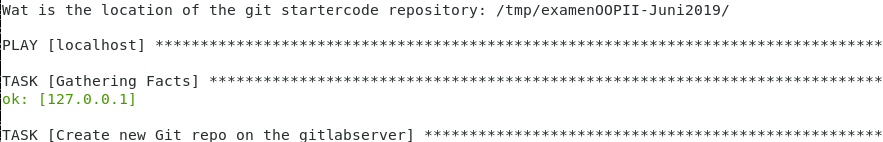
\includegraphics[width=\linewidth]{img/Git02.png}
   	\caption[Screenshot van het aanamken van een git repository met Ansible] {Hierboven zie je hoe het aanmaken van een gitlabproces geautomatiseerd is.}
   	\label{fig:PoC8}
   \end{figure} 
	\item Wanneer de studenten binnenkomen forken ze hun eigen private repository van het examenproject.
	
	   			\begin{figure}[H]
		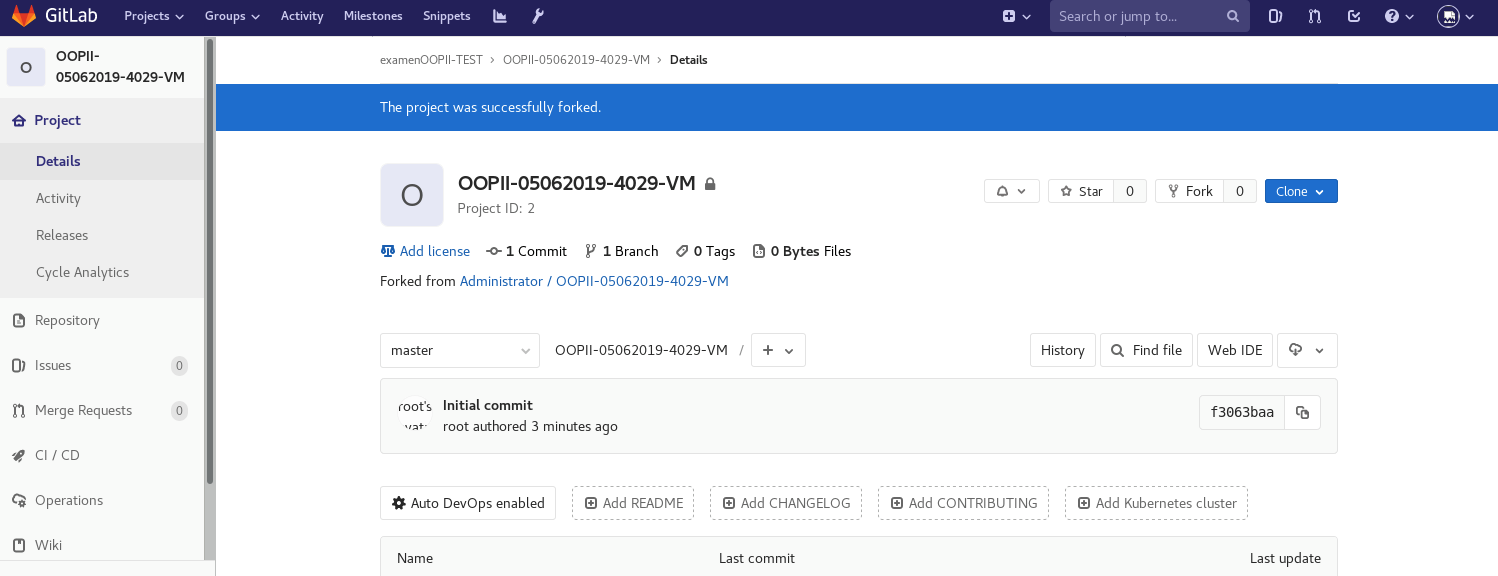
\includegraphics[width=\linewidth]{img/Fork1.png}
		\caption[Screenshot van een forked repository] {Hierboven zie je hoe de student een fork van de starterscode kan maken.}
		\label{fig:PoC9}
	\end{figure} 
	
	\item Tijdens het examen kunnen de studenten reeds pushen naar hun repository. Op het einde van het examen controleert de student of zijn oplossing correct op github staat.
	\item De Lector kan nu alle repositories van de studenten binnenhalen en verbeteren.
	   			\begin{figure}[H]
		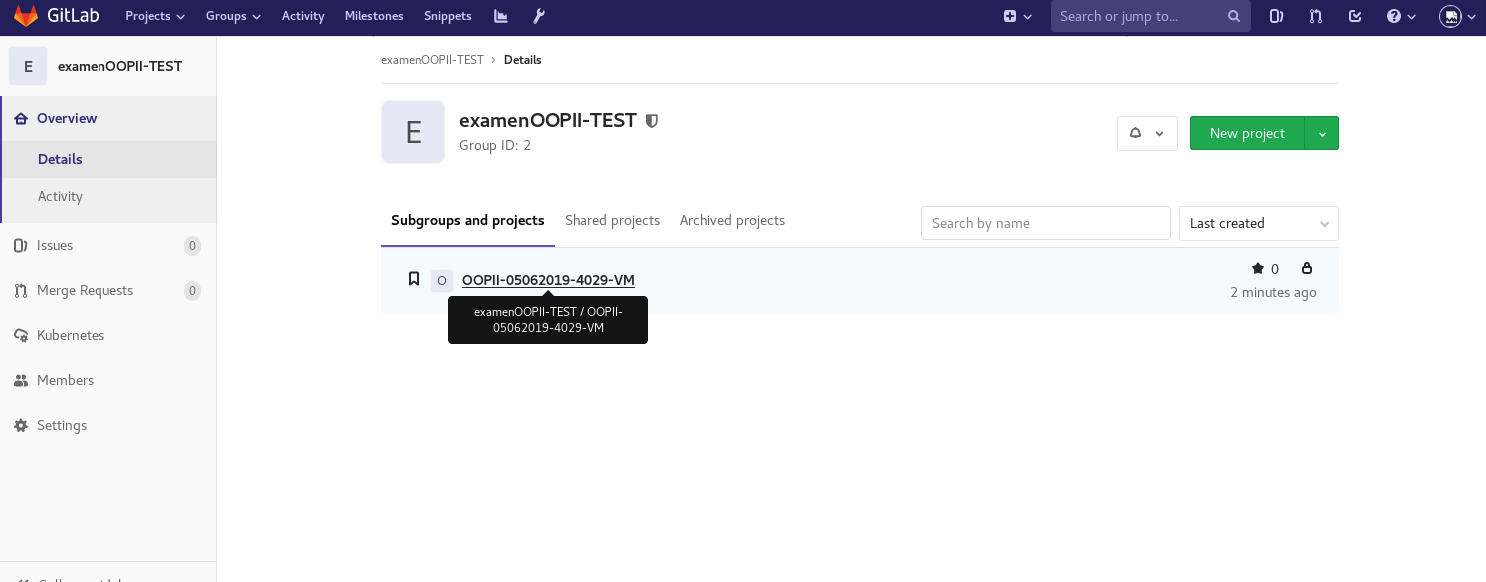
\includegraphics[width=\linewidth]{img/Check01.png}
		\caption[Screenshot van het overzicht die een lector heeft.] {Hierboven zie je wat de lector ziet na een examen, in dit geval heeft slechts 1 student een fork gemaakt}
		\label{fig:PoC10}
	\end{figure} 
	
	
\end{itemize}






% Voeg hier je eigen hoofdstukken toe die de ``corpus'' van je bachelorproef
% vormen. De structuur en titels hangen af van je eigen onderzoek. Je kan bv.
% elke fase in je onderzoek in een apart hoofdstuk bespreken.

%\input{...}
%\input{...}
%...

%%=============================================================================
%% Conclusie
%%=============================================================================

\chapter{Conclusie}
\label{ch:conclusie}

%% TODO: Trek een duidelijke conclusie, in de vorm van een antwoord op de
%% onderzoeksvra(a)g(en). Wat was jouw bijdrage aan het onderzoeksdomein en
%% hoe biedt dit meerwaarde aan het vakgebied/doelgroep? Reflecteer kritisch
%% over het resultaat. Had je deze uitkomst verwacht? Zijn er zaken die nog
%% niet duidelijk zijn? Heeft het onderzoek geleid tot nieuwe vragen die
%% uitnodigen tot verder onderzoek?





%%=============================================================================
%% Bijlagen
%%=============================================================================

\appendix

%%---------- Onderzoeksvoorstel -----------------------------------------------

\chapter{Onderzoeksvoorstel}

Het onderwerp van deze bachelorproef is gebaseerd op een onderzoeksvoorstel dat vooraf werd beoordeeld door de promotor. Dat voorstel is opgenomen in deze bijlage.

% Verwijzing naar het bestand met de inhoud van het onderzoeksvoorstel
%---------- Inleiding ---------------------------------------------------------

\section{Introductie} % The \section*{} command stops section numbering
\label{sec:introductie}

 Momenteel worden de meeste computerexamens op Hogeschool Gent in een beveiligde omgeving op een computer van de hogeschool afgenomen. Deze methodiek zorgt voor een hoge kost. De hogeschool moet een groot aantal computers te beschikking stellen. Deze moeten beschikken over software eigen aan het examen, en monitoringsoftware bevatten zodat examens in een beveiligde omgeving afgelegd kunnen worden. \\ In deze bachelorproef onderzoeken we de haalbaarheid van een beveiligde omgeving waar studenten computerexamens op hun eigen laptop kunnen afleggen. Deze beveilige omgeving moet maximaal vermijden dat fraude mogelijk is. \\

Deelonderzoeksvragen:
  \begin{itemize}
     \item Hoe gebeuren computerexamens nu op de hogeschool? Welke tools worden gebruikt? Welke regels en beperkingen leggen lectoren nu typisch op bij computerexamens?
     
     \item Welke tools/oplossingen bestaan er tegenwoordig voor dit soort situaties? Zijn die voldoende flexibel om bijvoorbeeld een examen programmeren of andere ict-vakken te faciliteren?
     
     \item Als we zelf een omgeving willen opzetten, welke componenten moet die dan bevatten? Welke beperkingen kunnen we studenten opleggen en welk gedrag kunnen we niet vermijden?
  \end{itemize}

%Hier introduceer je werk. Je hoeft hier nog niet te technisch te gaan.
%Je beschrijft zeker:
%\begin{itemize}
%  \item de probleemstelling en context
%  \item de motivatie en relevantie voor het onderzoek
%  \item de doelstelling en onderzoeksvraag/-vragen
%\end{itemize}

%---------- Stand van zaken ---------------------------------------------------

\section{Literatuurstudie}
\label{sec:literatuurstudie}

\subsection{Voordelen van bring-your-own-device examens}

Studenten die een examen afleggen op hun eigen hardware zijn vertrouwd met hun toestel. Waardoor hun stressgevoeligheid afneemt, volgens
 \textcite{TeckSwee2014}. In dat onderzoek was er op een populatie van 672 studenten 74.02\% blij met deze manier om examens af te nemen. 

\subsection{Problemen bij bring-your-own-device examens}
\subsubsection{Fraude}
Aangezien examens afleggen op eigen hardware een relatief nieuw gegeven is, ervaren we nog enkele kinderziektes.\\ \textcite{Dawson2016} bekeek in zijn onderzoek 5 manieren om fraude te plegen tijdens een examen op eigen laptop, namelijk: \\
\begin{itemize}
    \item De examenopgave lokaal opslaan en achteraf online plaatsen.
    \item Het examen op een virtuele omgeving afleggen en op die manier het besturingssysteem manipuleren
    \item Scripts uitvoeren via usb-keyboard hacks
    \item Software aanpassingen maken 
    \item Cold-boot aanval\\
\end{itemize}


Volgens het onderzoek van \textcite{VegendiaSindre2015} is het vermijden van elektronische communicatie een prioriteit. Dit is dan ook iets wat in de proof-of-concept onmogelijk gemaakt moet worden. 

\subsubsection{Overige problemen}

Naast fraude zijn er andere aandachtspunten bij het afnemen van examens op eigen hardware, \textcite{Hillier2015} heeft het in zijn onderzoek over onder andere: laptops die niet sterk genoeg zijn om bepaalde software aan te kunnen, onverwachte crashes van software of besturingssystemen, hardware die tijdens het examen faalt en batterijcapaciteit (indien er geen toegang tot stroom is). 



% Voor literatuurverwijzingen zijn er twee belangrijke commando's:
% \autocite{KEY} => (Auteur, jaartal) Gebruik dit als de naam van de auteur
%   geen onderdeel is van de zin.
% \textcite{KEY} => Auteur (jaartal)  Gebruik dit als de auteursnaam wel een
%   functie heeft in de zin (bv. ``Uit onderzoek door Doll & Hill (1954) bleek
%   ...'')


%---------- Methodologie ------------------------------------------------------
\section{Methodologie}
\label{sec:methodologie}

Voor dit onderzoek maken we een Analyse en beslissen we over de scope en de vereisten van de beveiligde omgeving. We gaan een onderzoek doen naar huidige oplossingen voor bring-your-own-device examens. \\ Via een rondvraag bij docenten gaan we onderzoeken welke vereisten elk computerexamen heeft. Zo kunnen we in de proof-of-concept een preset maken voor elk specifiek examen op computer. \\ De proof-of-concept zelf zal een volledig virtuele omgeving zijn, daarvoor gaan we o.a. gebruik maken van GNS3 en VirtualBox. 

%---------- Verwachte resultaten ----------------------------------------------
\section{Verwachte resultaten}
\label{sec:verwachte_resultaten}

Aan het einde van dit onderzoek verwachten we een compleet werkende en veilige proof-of-concept omgeving te hebben. De bedoeling is dat docenten hiermee vlot hun examens kunnen voorbereiden en verzekerd zijn van de fraudebestendigheid.


%---------- Verwachte conclusies ----------------------------------------------
\section{Verwachte conclusies}
\label{sec:verwachte_conclusies}

We verwachten dat een dergelijke omgeving op te zetten is. Al vrezen we wel dat er enkele beperkingen aan dit systeem zullen zijn. Bijvoorbeeld: aangezien het niet de bedoeling is dat er software op de laptop van een student geïnstalleerd wordt, zal je extra informatie die een student op zijn laptop zelf staan heeft niet kunnen verbieden. 




%\addcontentsline{toc}{chapter}{\textcolor{maincolor}{\IfLanguageName{dutch}{Bibliografie}{Bibliography}}}
%%---------- Andere bijlagen --------------------------------------------------

\chapter{Interviews}

Extra informatie werd verworven doormiddel van interviews met Docenten op Hogeschool Gent, Faculteit Bedrijf en Organisatie.


\section{Orientatie}

Momenteel wordt er naar 4 systemen gekeken voor dit onderzoek:
\begin{itemize}
	\item Safe Exam Browser 
	\item Televic AssessmentQ / AVIDAnet Lite
	\item Desktop virtualisatie via een cloudprovider
	\item Beveiligde, configureerbare netwerkomgeving om internettoegang tot niet-toegestane sites vanop laptops te vermijden
\end{itemize}
De vragen die gesteld worden tijdens dit interview zijn bedoeld om af te toetsen welk systeem het meest geschikt zou blijken volgens docenten om het huidige "systeem" met o.a. Netop School te vervangen. 
\newpage
\section{Vragen}

\begin{itemize}
	\item Neemt u computerexamens af op Hogechool Gent? Zoja, welke vakken? 
	\bigskip 
	\item Wat voor soort computerexamen neemt u af?
	\begin{itemize}
		\item Een online test waarbij antwoorden via de webbrowser invgevuld worden (bv. via Chamilo, Cisco-platform, enz.)
		\item Een schriftelijk examen waaarbij de voorbereiding op pc gebeurt maar de antwoorden op papier ingevuld worden.
		\item Een examen dat op computer m.b.v. specifieke software (bv. IDE en compiler) gemaakt wordt waarna het resultaat digitaal ingediend wordt (bv. Word document met antwoorden, zip-bestand met broncode, Github, ...)
		\item  Andere (te specifiëren)
		
	\end{itemize}
	\bigskip 

	\item Ik overloop nu enkele functies waarover een byod examensysteem zou kunnen beschikken. Kan u aangeven of deze essentieel (Must have), belangrijk, maar niet essentieel (Should have), nuttig, maar niet belangrijk (Could have) of onbelangrijk (Won't have) zijn?
	\begin{itemize}
		\item Toegang tot het internet kan verboden worden
		\item Beperken van toegang tot documenten
		\item Beperken van toegang tot software
		\item Digitale communicatie met medestudenten is niet mogelijk
		\item Monitoring tijdens het examen
		\item Snel en makkelijk opzetten van examens. 
		
\end{itemize}	
	\bigskip 
	\item Welke functies ontbreken momenteel de huidige manier waarop examens, op de computers van HoGent, afgenomen worden?
	\bigskip 
	\item Hoelang duurt het momenteel om een examen op computer voor te bereiden en hoe wordt dit gedaan (Computerlokaal voorbereiden, juiste examenfiles op de computer plaatsen) en hoe lang duurt het achteraf om alle examens op te halen?
	\bigskip 
	\item De huidige manier om examens af te leggen verloopt niet altijd zonder problemen. Kan u enkele defecten opsommen die u reeds tegengekomen bent? Moet u soms extra werk doen om alle examens op te halen (alle of enkele computers manueel afgaan)? Loopt er soms iets mis 10 minuten voor examen (softwarepaketten die ontbreken, examens die verdwenen zijn)? 
	\bigskip
	\item (Specifiek voor de docenten die programmeerexamens afleggern) Ziet u iets in het systeem van GitHub Classroom? Daarmee is het mogelijk om studenten gecontroleerd toegang te geven tot een opgave, een deadline op te leggen voor het indienen hiervan en zelfs automatisch te testen (m.b.v. een DevOps pipeline) en graden. Vergeleken met het huidige systeem (Word document) zou dit een veel meer efficiënte en veilige manier zijn.
	\bigskip 
	\item Heeft u nog vragen, Ideeën of opmerkingen over het nieuwe systeem?
	
\end{itemize}



%%---------- Referentielijst --------------------------------------------------

\printbibliography[heading=bibintoc]

\end{document}
